%%%%%%%%%%%%%%%%% DO NOT CHANGE HERE %%%%%%%%%%%%%%%%%%%% {
\documentclass[12pt,letterpaper]{article}
\usepackage{fullpage}
\usepackage[top=2cm, bottom=4.5cm, left=2.5cm, right=2.5cm]{geometry}
\usepackage{amsmath,amsthm,amsfonts,amssymb,amscd}
\usepackage{lastpage}
\usepackage{enumerate}
\usepackage{fancyhdr}
\usepackage{mathrsfs}
\usepackage{xcolor}
\usepackage{graphicx}
\usepackage{subcaption}
\usepackage{listings}
\usepackage{hyperref}
\usepackage{tikz}
\usepackage{ragged2e}
\usepackage{booktabs,tabularx}
\newcommand\mcc[1]{\multicolumn{2}{c}{#1}}
\usetikzlibrary{positioning,shapes,arrows}
\usetikzlibrary[calc]

\hypersetup{%
  colorlinks=true,
  linkcolor=blue,
  linkbordercolor={0 0 1}
}

\setlength{\parindent}{0.0in}
\setlength{\parskip}{0.05in}
%%%%%%%%%%%%%%%%%%%%%%%%%%%%%%%%%%%%%%%%%%%%%%%%%%%%%%%%%% }

%%%%%%%%%%%%%%%%%%%%%%%% CHANGE HERE %%%%%%%%%%%%%%%%%%%% {
\newcommand\course{CSI5138[F]: Intro: DL/RL}
\newcommand\semester{Fall 2019}
\newcommand\hwnumber{3}                 % <-- ASSIGNMENT #
\newcommand\NetIDa{Ao Zhang, 0300039680}           % <-- First Author
\newcommand\NetIDb{Lingfeng Zhang, 0300134245}           % <-- Second Author
%%%%%%%%%%%%%%%%%%%%%%%%%%%%%%%%%%%%%%%%%%%%%%%%%%%%%%%%%% }

%%%%%%%%%%%%%%%%% DO NOT CHANGE HERE %%%%%%%%%%%%%%%%%%%% {
\pagestyle{fancyplain}
\headheight 35pt
\lhead{\NetIDa}
\lhead{\NetIDa\\\NetIDb}                 
\chead{\textbf{\Large Assignment \hwnumber}}
\rhead{\course \\ \semester}
\lfoot{}
\cfoot{}
\rfoot{\small\thepage}
\headsep 1.5em
%%%%%%%%%%%%%%%%%%%%%%%%%%%%%%%%%%%%%%%%%%%%%%%%%%%%%%%%%% }

% Define block styles
\tikzstyle{sum} = [circle, draw, minimum size=1em]
\tikzstyle{mul} = [rectangle, draw, minimum size=1em]
\tikzstyle{var} = [text width=1em, text centered, minimum size=1em]
\tikzstyle{sig} = [diamond, draw, fill=blue!20, minimum size=1em]
\tikzstyle{sqsum} = [circle, draw, fill=blue!20, minimum size=1em]
\tikzstyle{line} = [draw, -latex’]

\begin{document}

\section{Data Processing}

\subsection*{Word Vector Representation}

Since the dataset contains totally $166971$ words in both training set and test set, the word embedding vector representation is required for the training, as the requirement says. Therefore, we first transfer the all the text files in the dataset into one text file, then we feed that text file into the GloVe. After training in the GloVe, a ``vocab.txt’’ and a ``vectors.txt’’ are created. Note that in this assignment, we use a vector sized $(1, 50)$ to represent a word.

Based on the files produced by GloVe, we first create a word dictionary into a python dictionary as format,
\begin{verbatim}
{
    str(word1) : 0,
    str(word2) : 1,
    …
}
\end{verbatim}
Then, we transfer every word in the dataset to an dictionary index. This immediately reduces the dataset size occupied in the RAM, which helps us train the model faster.

Similarly, we transfer the vector as a numpy array with format,
\begin{verbatim}
[[float, float, float, …, float, float],
[float, float, float, …, float, float],
…,]
\end{verbatim}
with the first axis standing for the index in the word dictionary. After such processing, each word in the dataset can be transferred into a digit array with size $(1, 50)$.

\subsection*{Maximum Sequence Length}

Since the length of each review in the dataset varies dramatically from each other, ranging from $4$ words to $2470$ words, we must set a limit length to filter the input to avoid feeding too many data into the model causing huge resource assumption.

A plot illustrating the distribution of file lengths is shown as Figure~\ref{fig:length}.
\begin{figure}[h]
    \centering
    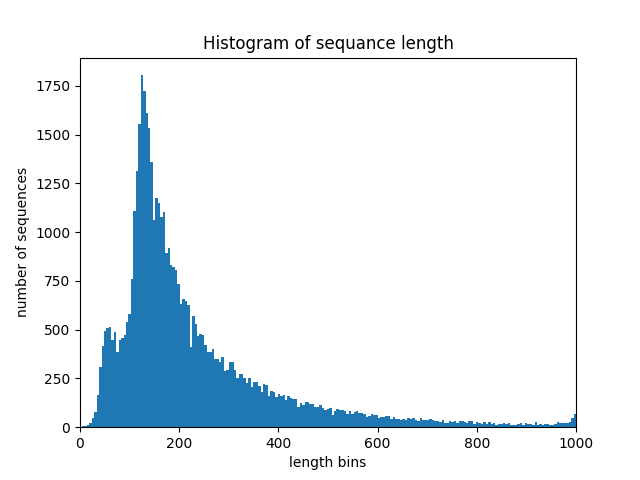
\includegraphics[width=.6\linewidth]{lengthdistribution.png}
    \caption{\small Distribution of dataset file lengths.}
    \label{fig:length}
\end{figure}

Clearly, most data files have length less than $400$. After weighting the loss of information of data itself and the efficiency of training the model, we finally set our length limit as $300$ words. So the number of kernels in RNN is 300. Vanilla RNN final state model with longer sequence length is prone to occur gradient vanishing and gradient exploding. Although mean pooling can reduce gradient vanishing but it do not work for gradient exploding. LSTM can work well for dealing with the problem of gradient exploding and gradient vanishing, but LSTM may occur gradient exploding sometimes.

One thing should be mentioned is: in order to get the fixed input length, we fill the input up with zeros if the data length is less than $300$, which is called sequence padding and truncate input length down to the maximum sequence length, which is called sequence truncation.

\section{Modelling}

First of all, the model is built with both TensorFlow API and Keras. As for the model with TensorFlow API all hyper-parameters are set as the following Table~\ref{T:parameters},
\begin{table}[h]
        \centering
        \vspace{\baselineskip}
        \caption{hyper-parameters settings.}\label{T:parameters}
      \begin{tabular}{cc}
        \hline
        Parameter & Value\\
        \hline
        sequence length limit & $300$\\
        batch size & $1000$\\
        epochs & $150$\\
        learning rate (start) & $0.001$\\
        learning rate decay rate & $0.96$\\
        test checking point & every $20$ steps\\
        classification function & softmax\\
        loss function & cross entropy\\
        optimizer & Adam\\
        \hline
      \end{tabular}
\end{table}
For each model, we tuned several values of the hyper-parameter \emph{learning rate decay steps} to get the stable results. Therefore, all the results we got are based on the different decay steps.

Second, in the assignment, we used one of the typical model introduced in the lecture (shown as Figure~\ref{fig:mode}),
\begin{figure}[h]
    \centering
    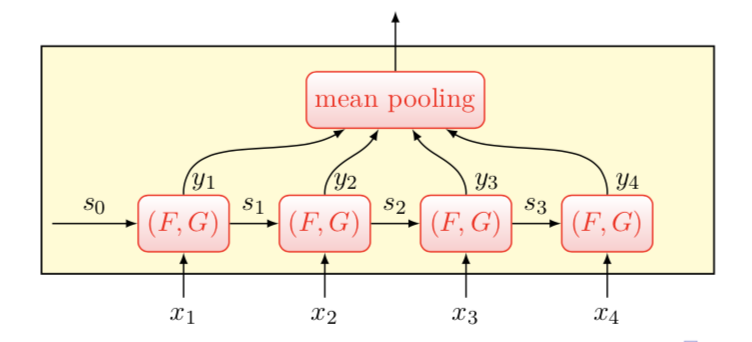
\includegraphics[width=.6\linewidth]{mode.png}
    \caption{\small Mean pool of the output.}
    \label{fig:mode}
\end{figure}

Mean pooling is a good method as the output of the model. First, since we have $300$ sequence steps, the sequence length is relatively long. When doing the back propagation in final state RNN model, it is easy to occur gradient vanishing because gradient is exponentially small if the largest eigenvalue of parameter matrix $W_h$ is less than one. If the mean pooling RNN model is applied, the prior gradient will not easily be vanishing, so the total gradient is not vanishing and mean pooling RNN model can keep more information. This is the reason why, as experiments show, in such cases, the mean pooling performs better than only extract last output as the output of model.

\section{Results}

In this session, we will go first into the comparison of the performances of different models, then we will show the results of the influence of the model complexities.

\subsection*{Vanilla RNN and LSTM}

The comparison of Vanilla RNN and LSTM are shown as Figure~\ref{fig:comparison}. below.
\begin{figure}[h]
    \begin{subfigure}{0.4\textwidth}
    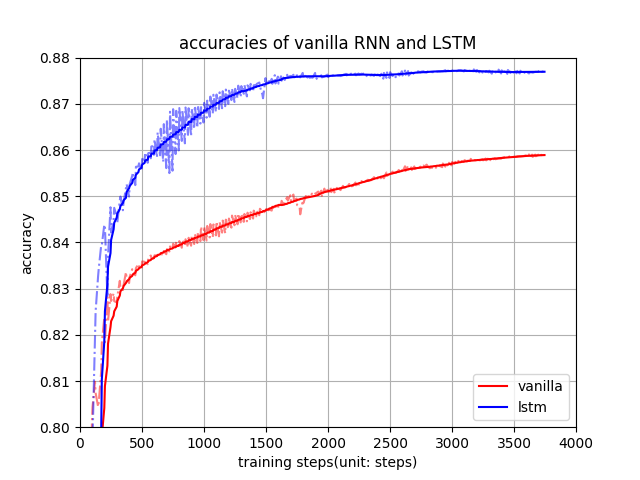
\includegraphics[width=\linewidth]{compare_acc.png}
    \caption{\small Accuracy of Vanilla RNN and LSTM with state dimension $50$.} \label{fig:a}
    \end{subfigure}\hspace*{\fill}
    \begin{subfigure}{0.4\textwidth}
    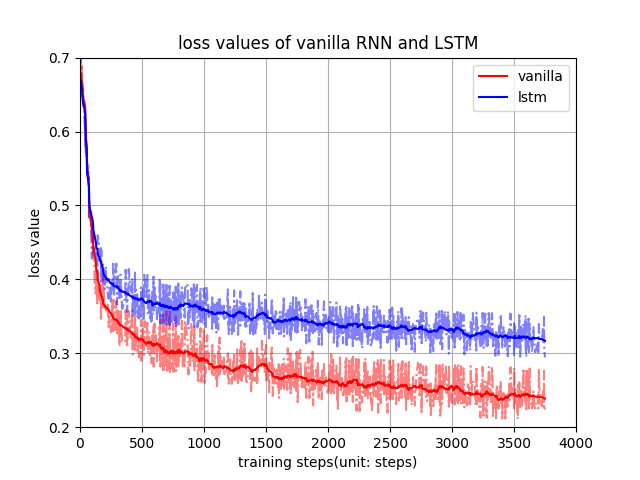
\includegraphics[width=\linewidth]{compare_loss.png}
    \caption{\small Loss value of Vanilla RNN and LSTM with state dimension $50$.} \label{fig:b}
    \end{subfigure}
    \caption{Compare Vanilla RNN and LSTM.}
    \label{fig:comparison}
\end{figure}

For a brief conclusion, it is obvious that the LSTM outperforms the Vanilla RNN, although the loss value of the LSTM is generally higher than the Vanilla. The main reason is that the LSTM contains more parameters which amplify the loss value.

\subsection*{Influence of the State Dimension}

First of all, let us use some graphs(see Figure~\ref{fig:state_dim}.) to illustrate the overall influence of the state dimension. These graphs are tuned well to avoid gradient vanishing and exploding.
\begin{figure}[h]
    \begin{subfigure}{0.49\textwidth}
    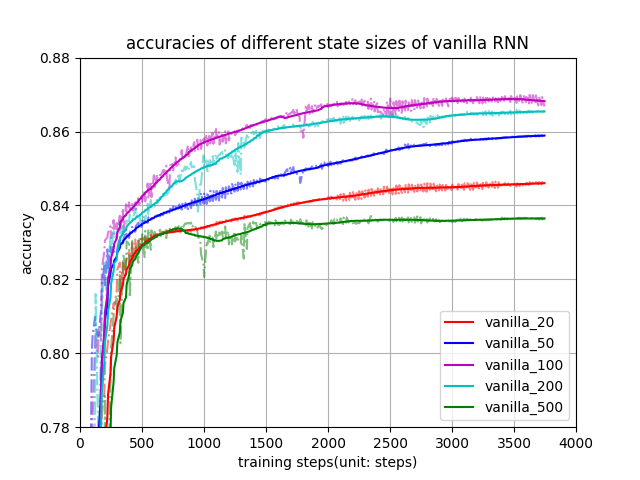
\includegraphics[width=\linewidth]{vanilla_acc.png}
    \caption{\small Results on accuracy of Vanilla RNN.} \label{fig:a}
    \end{subfigure}\hspace*{\fill}
    \begin{subfigure}{0.49\textwidth}
    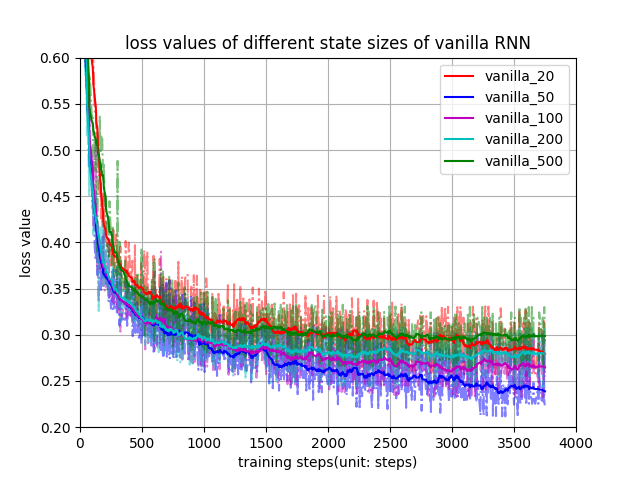
\includegraphics[width=\linewidth]{vanilla_loss.png}
    \caption{\small Results on loss of Vanilla RNN.} \label{fig:b}
    \end{subfigure}
    
    \medskip
    \begin{subfigure}{0.49\textwidth}
    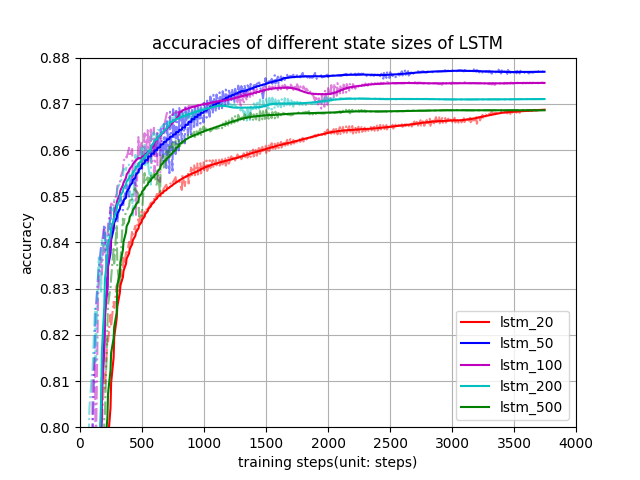
\includegraphics[width=\linewidth]{lstm_acc.png}
    \caption{\small Results on accuracy of LSTM.} \label{fig:c}
    \end{subfigure}\hspace*{\fill}
    \begin{subfigure}{0.49\textwidth}
    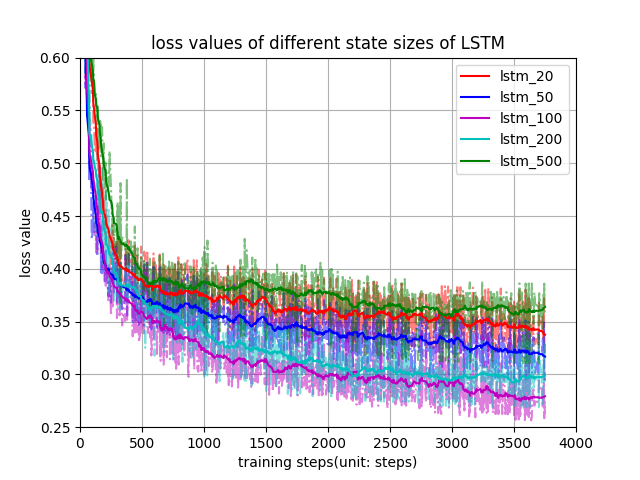
\includegraphics[width=\linewidth]{lstm_loss.png}
    \caption{\small Results on loss of LSTM.} \label{fig:d}
    \end{subfigure}
    \caption{Influence of state dimensions on $2$ models.} \label{fig:state_dim}
\end{figure}

Apparently, increasing the state dimension does not always improve the training speed and final test results. On the contrary, the performance goes up from dimension $20$ to $50$ at the beginning. Then, it starts showing that further increase of the dimension may worsen the model performance.

In order to find further influence of the state dimension on the model, also in order to meet the requirements of our assignment, a table is built showing the final stable results of models(see Table \ref{T:different_state_dim_results}).
\begin{table*}[!ht]
        \caption{Final results.}\label{T:different_state_dim_results}
        \centering
        \setlength{\tabcolsep}{4pt}
        \begin{tabularx}{\textwidth}{>{\hsize=1.9\hsize\bfseries\RaggedRight}X!{\extracolsep{\fill}}*{6}{>{\centering\arraybackslash\hsize=0.48\hsize}X}}
                \toprule[1pt]\midrule[0.3pt]
                \multicolumn{5}{c}{\textbf{Metrics Comparisons}} \\ \midrule[0.3pt]
                \textbf{Model}& \multicolumn{1}{c}{\textit{Vanilla RNN}} & \multicolumn{1}{c}{\textit{LSTM}} \\
                \cmidrule(lr){2-3} %\cmidrule(lr){4-5} %\cmidrule(lr){6-7}%
                {Metrics} & $accuracy$ & $accuracy$ \\
                \addlinespace%
                {State Size $20$} & 84.56\% & 86.86\% \\
                \addlinespace%
                {State Size $50$} & 85.91\% & 87.71\% \\
                \addlinespace%
                {State Size $100$} & 86.67\% & 87.44\% \\
                \addlinespace
                {State Size $200$} & 86.54\% & 87.10\% \\
                \addlinespace
                {State Size $500$} & 83.65\% & 86.86\% \\
                \midrule
                % \multicolumn{7}{c}{\textbf{XYZ Metrics}} \\ \midrule[0.3pt]
                % \textbf{Algorithm}& \multicolumn{2}{c}{\textit{Algo 1}} & \multicolumn{2}{c}{\textit{Algo 2}} & \multicolumn{2}{c}{\textit{Algo 3}} \\
                \cmidrule(lr){2-3} \cmidrule(lr){4-5}% \cmidrule(lr){6-7}%
                % {Average} & \multicolumn{1}{c}{10} & \multicolumn{1}{c}{0} \\ \addlinespace
                % {Matric 6} & \multicolumn{2}{c}{0} & \multicolumn{2}{c}{0} & \multicolumn{2}{c}{0} \\
                \midrule[0.3pt]\bottomrule[1pt]
        \end{tabularx}
\end{table*}

A figure \ref{fig:final acc} is also produced in order to make the results more easily to be visualized.
\begin{figure}[h]
    \begin{subfigure}{0.49\textwidth}
    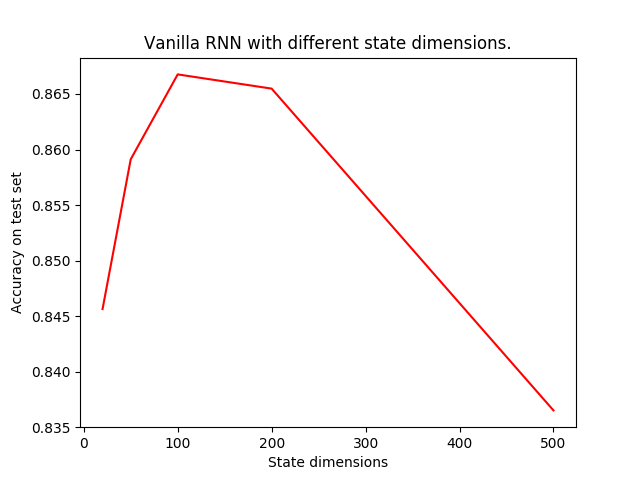
\includegraphics[width=\linewidth]{vanilla_final_acc.png}
    \caption{\small State dimensions on Vanilla RNN.} \label{fig:e}
    \end{subfigure}\hspace*{\fill}
    \begin{subfigure}{0.49\textwidth}
    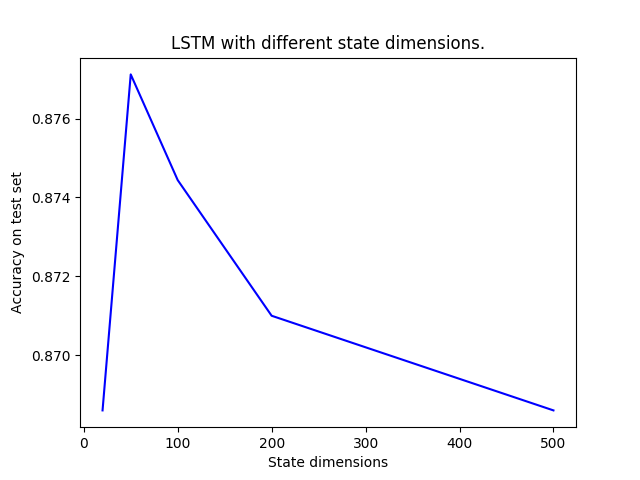
\includegraphics[width=\linewidth]{lstm_final_acc.png}
    \caption{\small State dimensions on LSTM.} \label{fig:f}
    \end{subfigure}
    \caption{Influence of state dimensions on $2$ models' accuracy.}
    \label{fig:final acc}
\end{figure}

By reviewing all the results above, one can conclude that: there exists an optimal solution on the state dimensions of RNN families when given a specific dataset. Other state dimensions on both side of the optimal one may not perform as well as the optimal solution. Therefore, in order to choose the best solution for state dimensions, one may conduct several experiments on the specific RNN model.

\section{Some experiments about different RNN models}

To understand RNN models deeply, we have done several experiments without tuning to find some interesting conclusions.

\begin{figure}[h]
    \begin{subfigure}{0.49\textwidth}
    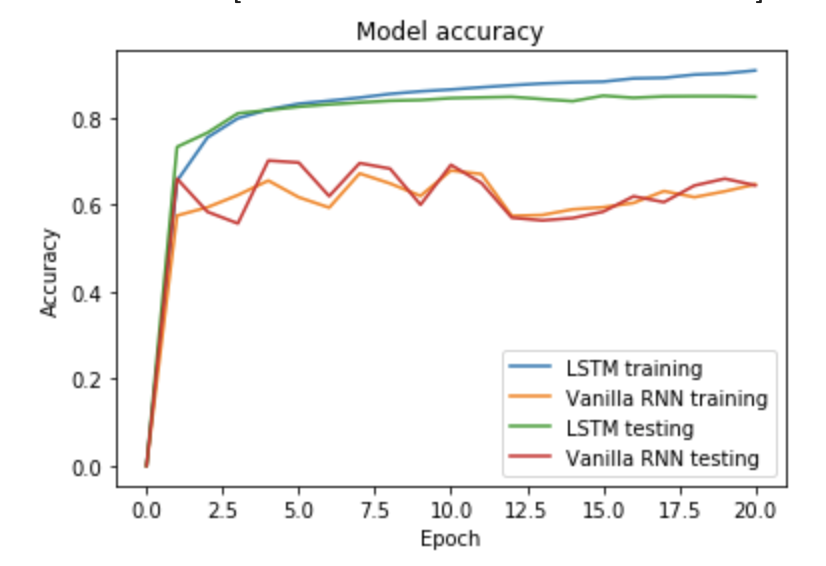
\includegraphics[width=\linewidth]{final_state_2_models.png}
    \caption{\small Comparing Vanilla RNN and LSTM based on final state.} \label{fig:e}
    \end{subfigure}\hspace*{\fill}
    \begin{subfigure}{0.49\textwidth}
    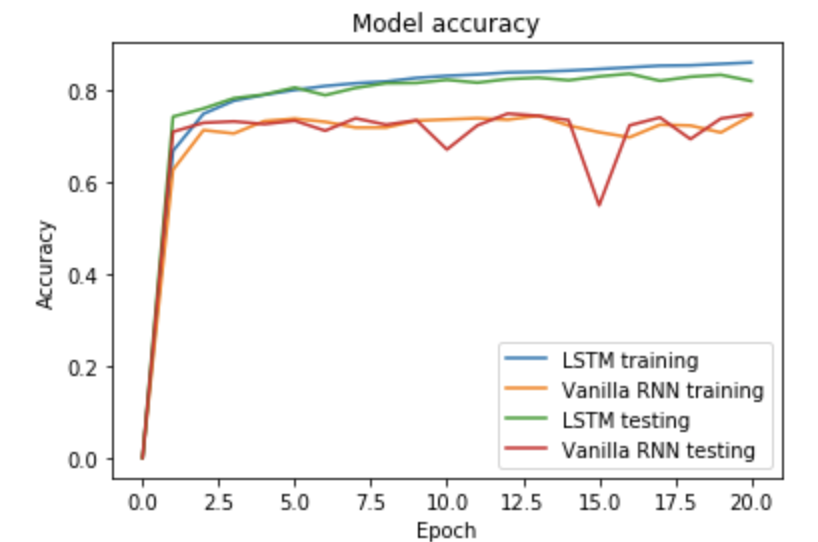
\includegraphics[width=\linewidth]{mean_pool_2_models.png}
    \caption{\small Comparing Vanilla RNN and LSTM based on mean pooling.} \label{fig:f}
    \end{subfigure}
    \caption{Comparing Vanilla RNN and LSTM based on extracting mean pooling and final state.}
    \label{fig:meanpool&finalstate}
\end{figure}

By comparing Vanilla RNN and LSTM based on extracting mean pooling and final state(see Figure~\ref{fig:meanpool&finalstate}), we see both extracting mean pooling and final state in Vanilla RNN are all gradient exploding sometimes, which is the disadvantage of Vanilla RNN, and LSTM can fix this problem up well. LSTM is more complex than Vanilla RNN and it seldom occur gradient exploding and vanishing, so its accuracy is higher than that of Vanilla RNN.

In these graphs, sometimes testing accuracy is higher than training accuracy. There are several reasons to interpret this phenomenon. First reason is training accuracy is measured during each epoch while testing accuracy is measured after each epoch. Another reason is the validation set maybe easier than the training set or their data distribution are not same. This happens when testing set is smaller than training set or was not properly sampled because these experiments' testing data worked as validation data(smaller than training dataset).Training set was divided into training data and validation data to save training time in these experiments. Another reason is data leakage happens, meaning training samples getting accidentally mixed in with validation samples.

The accuracy of mean pooling Vanilla RNN is higher than the one of final state. One reasonable way to illustrate this phenomenon is mean pooling can keep more information than extracting final state and mean pooling can reduce gradient vanishing. 

\begin{figure}[h]
    \begin{subfigure}{0.32\textwidth}
    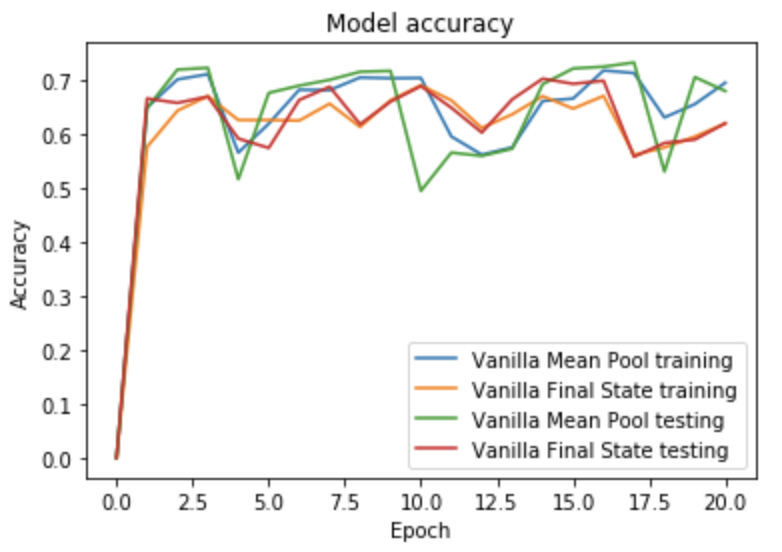
\includegraphics[width=\linewidth]{vanilla_compare_final&meanpool_1.png}
    \caption{\small Experiment 1} \label{fig:e}
    \end{subfigure}\hspace*{\fill}
    \begin{subfigure}{0.32\textwidth}
    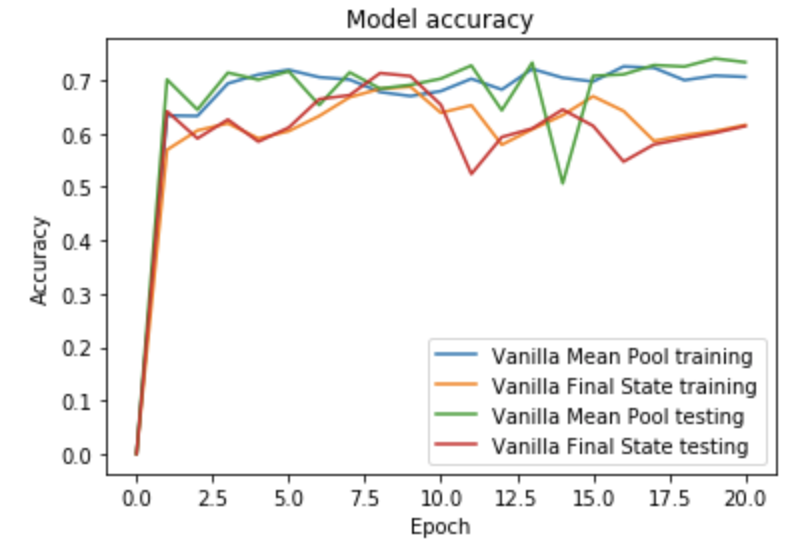
\includegraphics[width=\linewidth]{vanilla_compare_final&meanpool_2.png}
    \caption{\small Experiment 2} \label{fig:f}
    \end{subfigure}
    \begin{subfigure}{0.32\textwidth}
    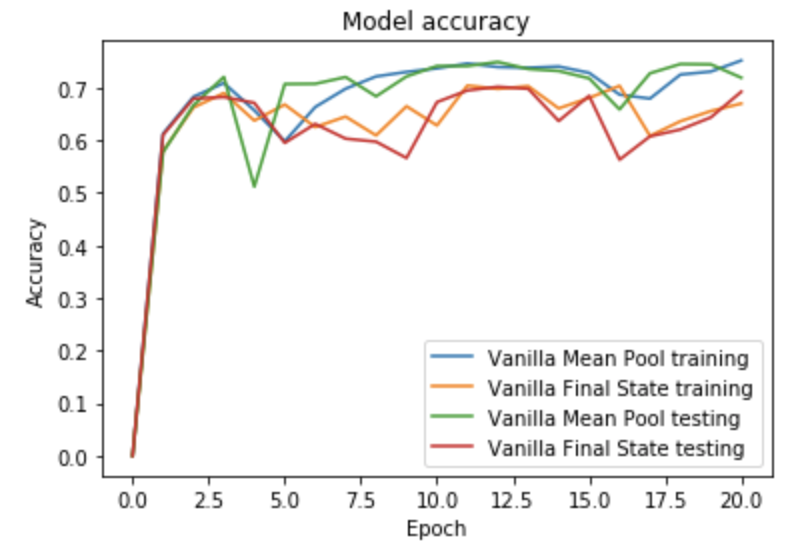
\includegraphics[width=\linewidth]{vanilla_compare_final&meanpool_3.png}
    \caption{\small Experiment 3} \label{fig:f}
    \end{subfigure}
    \caption{Comparing mean pooling and final state in vanilla RNN.}
    \label{fig:3_experiments_Vanilla}
\end{figure}

To verify this phenomenon, three experiments are done(see Figure~\ref{fig:3_experiments_Vanilla}). If less gradient exploding happening, extracting mean pooling can perform well than final state.

\begin{figure}[h]
    \centering
    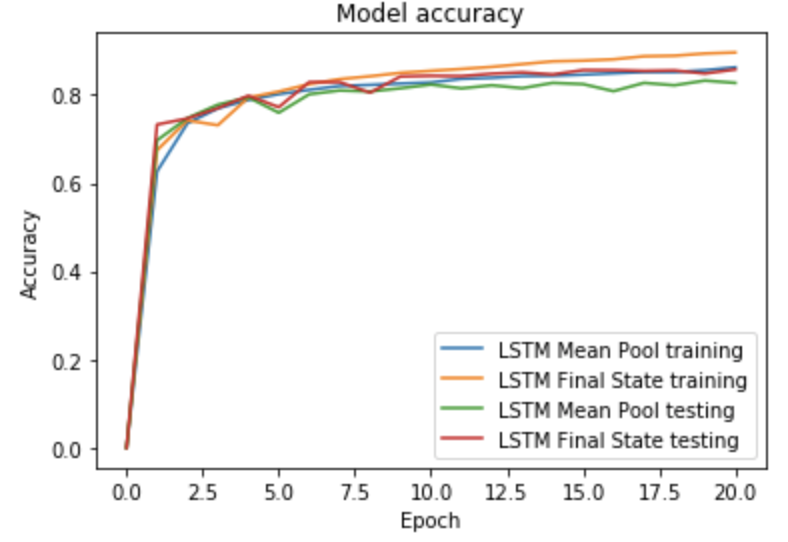
\includegraphics[width=.5\linewidth]{lstm_compare_final&meanpool.png}
    \caption{\small Comparing final state and mean pooling in LSTM}
    \label{fig:lstm_comparison}
\end{figure}

In addition, by comparing final state and mean pooling in LSTM, their accuracy are nearly same, but the accuracy of final state LSTM is slightly higher than the one of mean pooling(see Figure~\ref{fig:lstm_comparison}). This is possibly because mean pooling extracting too much information than needed.

\begin{figure}[h]
    \begin{subfigure}{0.49\textwidth}
    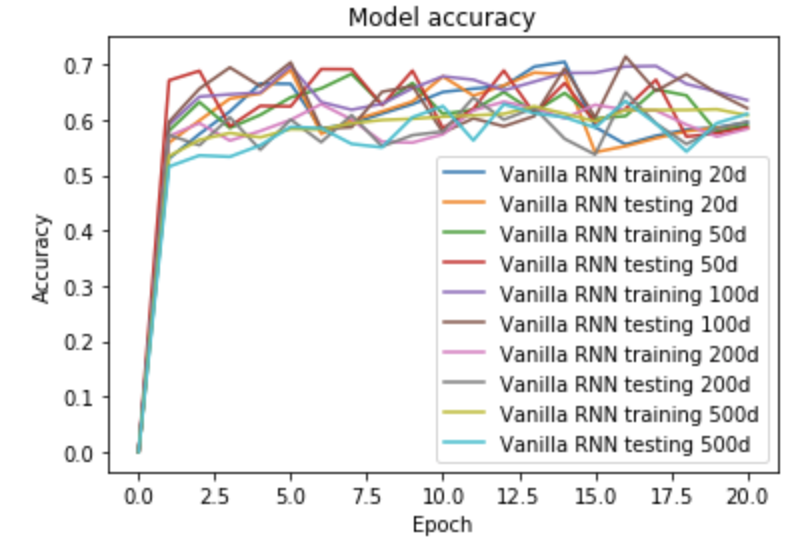
\includegraphics[width=\linewidth]{different_dim_vanilla_final_state.png}
    \caption{\small Extracting final state.} \label{fig:e}
    \end{subfigure}\hspace*{\fill}
    \begin{subfigure}{0.49\textwidth}
    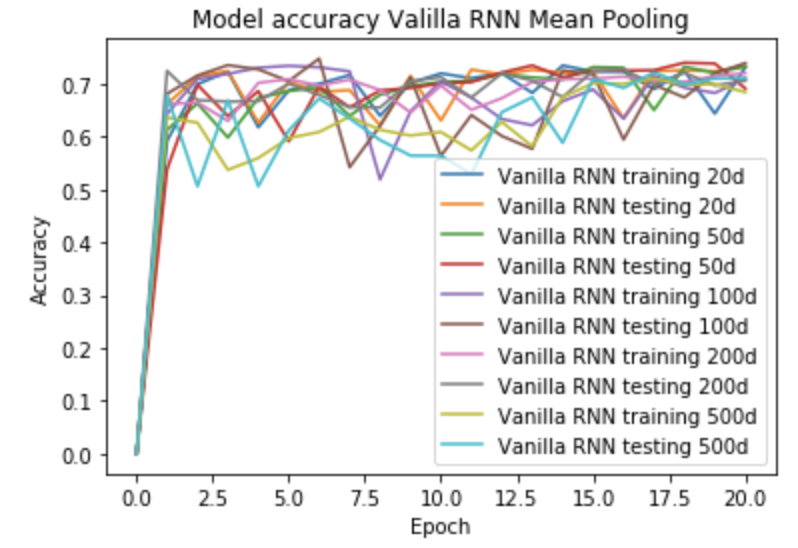
\includegraphics[width=\linewidth]{different_dim_vanilla_mean_pool.png}
    \caption{\small Extracting mean pooling.} \label{fig:f}
    \end{subfigure}
    \caption{Comparing different state dimension in Vanilla RNN}
    \label{fig:Vanilla_diffe_dim}
\end{figure}

Since gradient exploding happens frequently in Vanilla RNN, different state dimension comparison in Vanilla RNN whether using meal pooling or final state extraction could not access easily without tuning hyper-parameters(See Figure~\ref{fig:Vanilla_diffe_dim}).

Vanilla RNN with extracting final state is harder to tune than mean pooling, so tuned comparison model with mean pooling Vanilla RNN is shown in Figure~\ref{fig:state_dim} (a).

\begin{figure}[h]
    \begin{subfigure}{0.49\textwidth}
    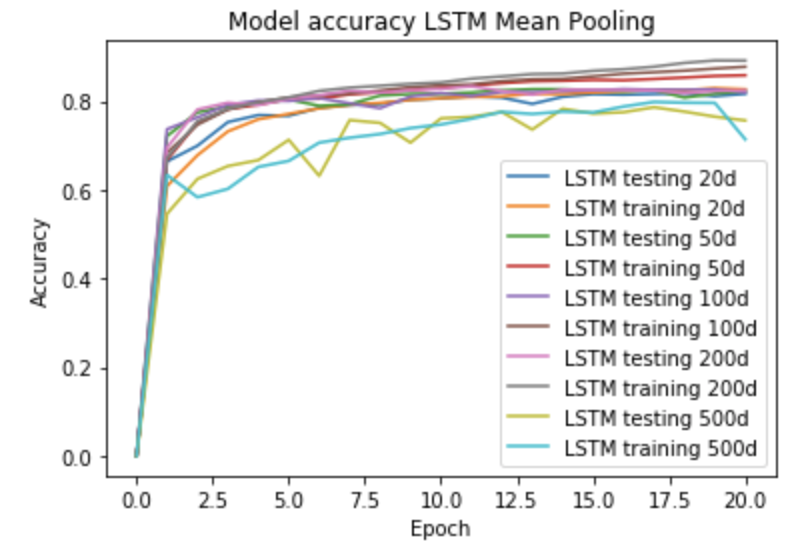
\includegraphics[width=\linewidth]{different_dim_lstm_mean_pool_1.png}
    \caption{\small LSTM with gradient exploding} \label{fig:e}
    \end{subfigure}\hspace*{\fill}
    \begin{subfigure}{0.49\textwidth}
    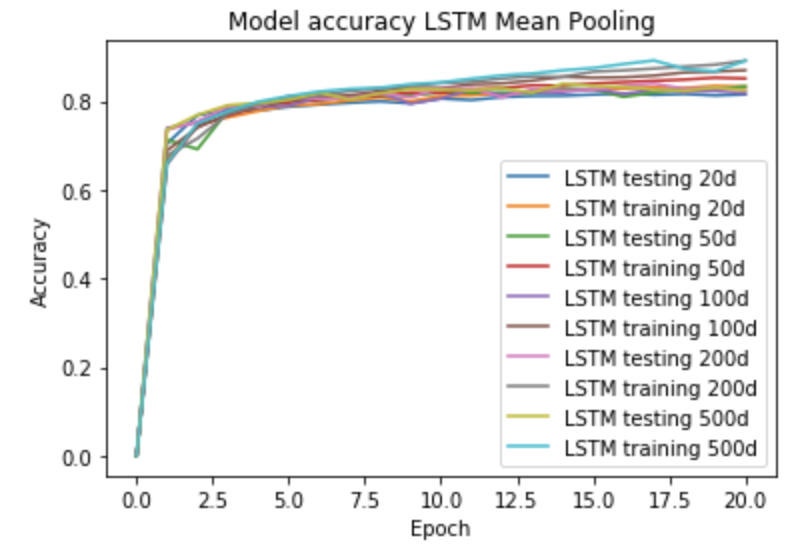
\includegraphics[width=\linewidth]{different_dim_lstm_mean_pool_2.png}
    \caption{\small LSTM without gradient exploding} \label{fig:f}
    \end{subfigure}
    \caption{Comparing different state dimension in mean pooling LSTM}
    \label{fig:LSTM_gradient_exploding}
\end{figure}

LSTM may occur gradient exploding too, although the possibility is extremely small. In Figure~\ref{fig:LSTM_gradient_exploding}(a), gradient exploding happens in 500 state dimension, when it trained again, gradient exploding vanished(see Figure~\ref{fig:LSTM_gradient_exploding}(b)).

\begin{figure}[h]
    \begin{subfigure}{0.49\textwidth}
    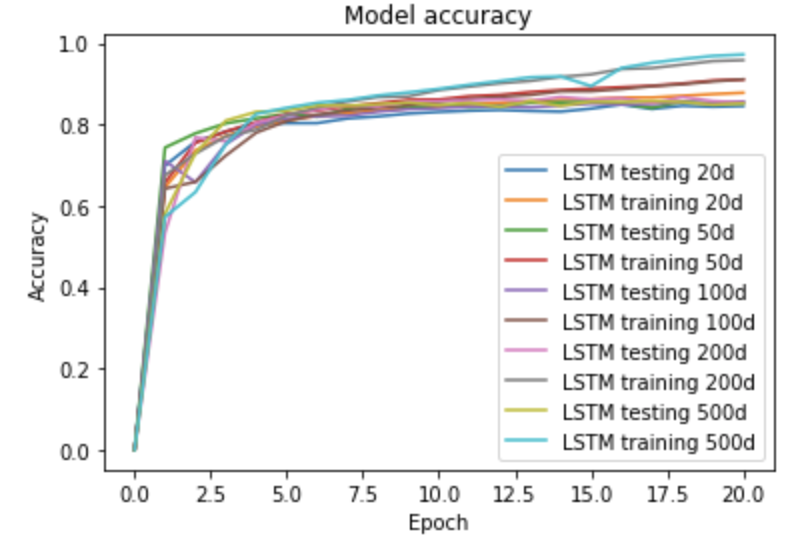
\includegraphics[width=\linewidth]{different_dim_lstm_final_state.png}
    \caption{\small final state LSTM} \label{fig:e}
    \end{subfigure}\hspace*{\fill}
    \begin{subfigure}{0.49\textwidth}
    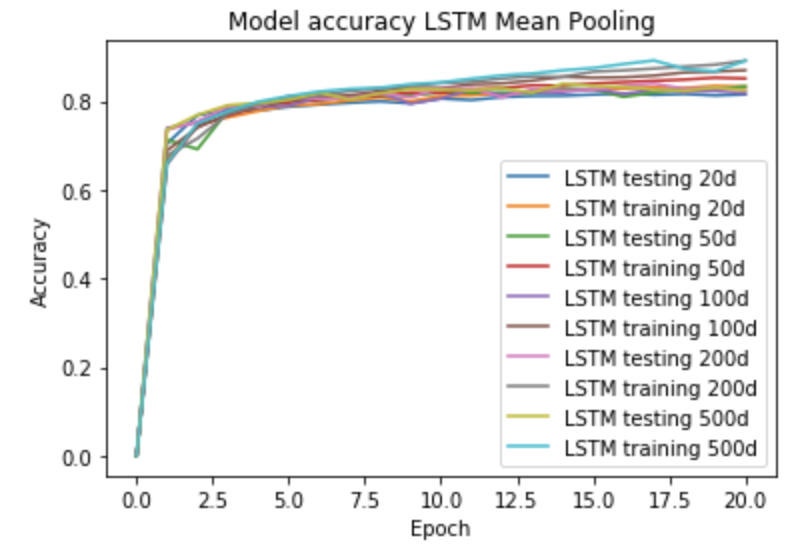
\includegraphics[width=\linewidth]{different_dim_lstm_mean_pool_2.png}
    \caption{\small mean pooling LSTM} \label{fig:f}
    \end{subfigure}
    \caption{Comparing different state dimension in two LSTM models}
    \label{fig:LSTM_differ_state_dim}
\end{figure}

By comparing different state dimension both in final state LSTM and mean pooling LSTM(see Figure~\ref{fig:LSTM_differ_state_dim}), it is shown that the model occur overfitting too much and the training accuracy increase of model with state dimension climbing. This is because when state dimension increasing, more parameters should be learned, the model become more complex, and training accuracy increases as well as overfitting occurs finally. 

\end{document}

